\documentclass{beamer}
\usepackage{amsmath}
\usepackage{enumitem}
\usepackage{url}

% put bullets back in font package
\setlist[itemize,1]{label={\fontfamily{cmr}\fontencoding{T1}\selectfont\textbullet}}

% remove stupid navigation tools and add page numbers
\mode<presentation>{\usetheme{Malmoe}}
\setbeamertemplate{navigation symbols}{}

\addtobeamertemplate{navigation symbols}{}{%
    \setbeamercolor{footline}{fg=black}
    \usebeamerfont{footline}%
    \usebeamercolor[fg]{footline}%
    \hspace{1em}%
    \insertframenumber/\inserttotalframenumber
}

\newcommand{\ignore}[1]{}
\newcommand*{\diff}{\mathsf{d}}
\newcommand{\some}{{\color{red} something}}
\renewcommand{\vec}[1]{\mathbf{#1}}
\newcounter{mybox}
\newcommand\ColorBox[2][]{%
\stepcounter{mybox}%
\node[draw=blue,fill=blue!20,align=left,#1] (box\themybox) {#2};
}

\title[Freezing a WCA Fluid using cDFT]{Freezing of a Weeks-Chandler-Anderson 
       Fluid using Classical Density Functional Theory}
\author{OSU Open House Presentation by Kirstie Finster} 
\date{March 12, 2021}

%%% DOCUMENT %%%

\begin{document}
\setbeamercolor{whitebox}{bg=gray!40}

%%main

\begin{frame}
	\titlepage
	%\center Dr. Roundy's Research Group in Computational Physics
\end{frame}


\section*{WCA Fluid}

\subsection*{Weeks-Chandler-Anderson (WCA) Model Fluid}
\begin{frame}{The WCA Model Fluid}
	\begin{columns}[t]
       \column{.5\textwidth}
       	\vspace{-1.5em}
		%\begin{block}{Real Liquids}
			%\begin{itemize}
			    %\item Model fluids help us 
			    
			    %understand real fluids
				%\item Short range repulsion 
				%\item Long range attraction 
			%\end{itemize}
		%\end{block}
		\begin{block}{}
			\begin{itemize}
			    \item Classical model fluid
				\item Soft, short range repulsion
                \item Slightly "squishy" spheres
				\item Exists in solid crystalline state when the free 
				energy it $\italic{would}$ have as a  solid is lower than the free 
				energy it $\italic{would}$ have as a fluid at that same temperature and density
				%\item Forms FCC crystals				
			\end{itemize}
		\end{block}		
		\column{.5\textwidth}
		\vspace{-3em}
          \begin{figure}
             \centering
             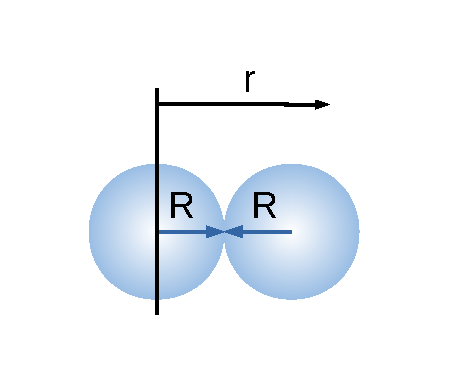
\includegraphics[width=1.1\columnwidth]{figs/TwoSpheresandplot.pdf} 
          \end{figure} 	 
	\end{columns}	
\end{frame}

%\subsection*{Freezing}

%\begin{frame}{Freezing of a WCA Fluid}
	%\begin{columns}[t]
		%\column{.5\textwidth}
	    %\vspace{-1em}
		%\begin{block}{Phase Transitions}
		     %\begin{itemize}
				%%\item Driven by entropy - maximize the entropy of the universe				
				%\item Abrupt change in density
				
				%across coexistence region
			 %\end{itemize}		
		%\end{block} 
		%\begin{block}{WCA Phase Diagram}
		     %\begin{itemize}
				%\item No attraction	- so no
				
				%liquid/gas boundary
				%\item Fluid is homogeneous (has
				
				%uniform average n spatially) 
				%\item "Solid" is a strongly 
				
				%inhomogeneous fluid 
				
				%with long-range order		
			  %\end{itemize}				 
		%\end{block}			       
		%\column{.5\textwidth}
	    %\vspace{-2em}
		 %\begin{figure}
            %\centering
            %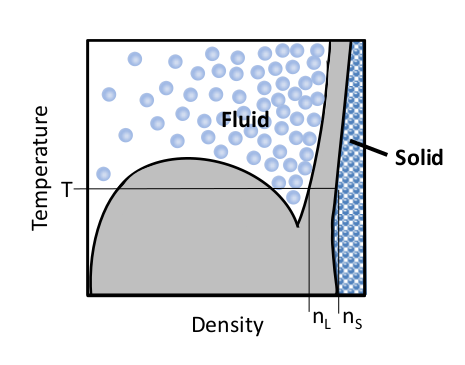
\includegraphics[width=1.1\columnwidth]{figs/T-n_Diagram.pdf}
          %\end{figure}
          %\vspace{-1em}
         %$~~~~~~~~~~$ T-n Phase Diagram  
       
	%\end{columns}
    %\vspace{+1em}
%\end{frame}

%\begin{frame}{Freezing of a WCA Fluid}
	%\begin{columns}[t]
		%\column{.5\textwidth}
	    %\vspace{-0.5em}
         %\begin{block}{At Phase Transition}
		     %\begin{itemize}
				%\item Thermal equilibrium 
				
				%($\text{T}_{Liquid}$ = $\text{T}_{Solid}$)
			    %\item Mechanical equilibrium 
			    
			    %($\text{P}_{Liquid}$ = $\text{P}_{Solid}$)
				%\item Diffusive equilibrium 
				
				%($\mu_{Liquid}$ = $\mu_{Solid}$)
			%\end{itemize}		
		%\end{block}	
		%\begin{block}{WCA Phase Diagram}
		     %\begin{itemize}
				%\item No liquid/gas boundary				
			  %\end{itemize}				 
		%\end{block}	
		%\column{.5\textwidth}
	    %\vspace{-1.5em}
		%\begin{figure}
            %\centering
            %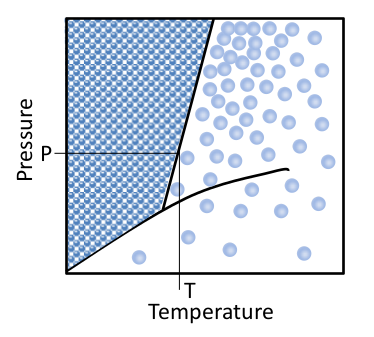
\includegraphics[width=\columnwidth]{figs/P-T_Diagram.pdf}
         %\end{figure} 
	    %\vspace{-1em}                  
         %$~~~~~~~~~~$P-T Phase Diagram
	%\end{columns}
    %\vspace{+1em}	
%\end{frame}

%\subsection*{Finding coexistence}
%\begin{frame}{Find Pressure and Number Densities at  Phase Transition}
	%\begin{columns}[t]
		%\column{.5\textwidth}
		%\vspace{-2em}
		%\begin{block}{}
			   %%\begin{displaymath}{P = -\frac{\partial{f}}{\partial{\frac{1}{n}}}\bigg|_{T,N}}\end{displaymath} 
				%%\begin{displaymath} \mu = f + \frac{1}{n}P\end{displaymath}
			%\begin{itemize} 
                 %\item Phase transition pressure at point where $P_L=P_S$ and $\mu_L=\mu_S$ for a given T							
			     %%\item Phase transition liquid and solid number densities found at phase transition pressure
			     %%item Find Helmholtz free energy
			     %\vspace{+1em}
			     %\item Helmholtz free energy per atom, $f=\frac{F}{N}$ at T, n gives

				 %%\item %Pressure = -slope								
				 %\begin{displaymath}{P = -\frac{\partial{f}}{\partial{\frac{1}{n}}}\bigg|_{T,N}}\end{displaymath} 
				 %%\item %$\mu$ = y-intercept
				 %\begin{displaymath} \mu = f + \frac{1}{n}P\end{displaymath}		
				 %Find pressure at intersection 		
			%\end{itemize}
	    %\end{block}	    
	    %\column{.55\textwidth}
		%\vspace{-2em}
            %\begin{figure}
                %\centering
                %%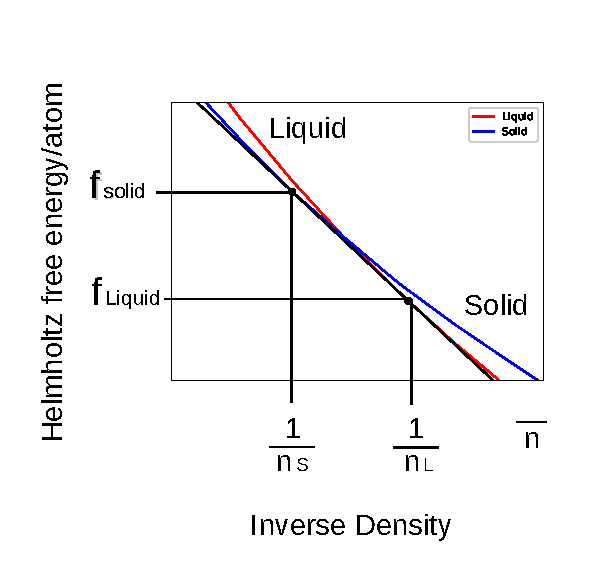
\includegraphics[width=1.2\columnwidth]{figs/MaxwellDTC-Fig1-realplot.pdf}
                %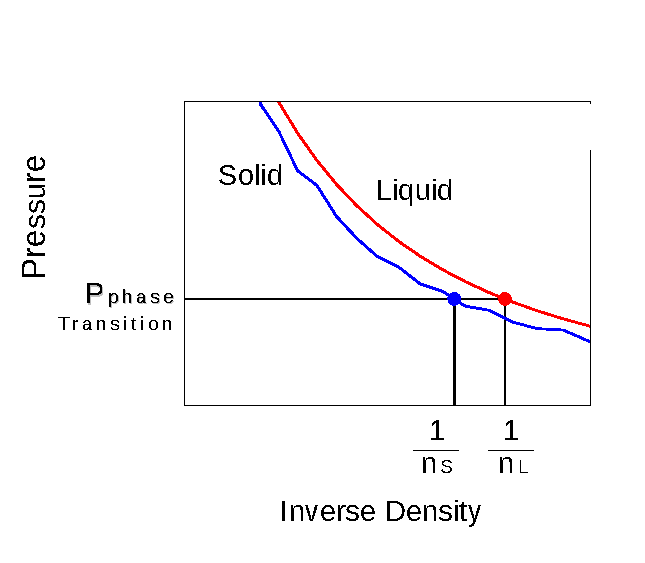
\includegraphics[width=0.9\columnwidth]{figs/MaxwellDTC-Fig3-realplot.pdf}
            %\end{figure}
            %\vspace{-.5em}
			%\begin{itemize} 						
			    %\item Phase transition liquid and solid number densities, $\text n_L$ and $\text n_S$ found at $\text P_{phase.transition}$
			%\end{itemize}
            
            %%\textcolor{blue}{$~~~~~~~~~~~\rightarrow$ Find Helmholtz free energy}
	%\end{columns}	
%\end{frame}


\section*{Classical Density Functional Theory (cDFT)}
\subsection{Find Freezing using cDFT}
\begin{frame}{To find freezing at a given temperature and number density using cDFT...}
%\begin{block}{}
     \large
     \center Express Helmholtz free energy as a functional  
     \center $\text{F}[n(\vec r)]$ 
     %\center of the number density profile $n(\vec r)$ 
     \center of the average single particle number density $n(\vec r)$
     \normalsize
     %\vspace{-1em}
      %The Helmholtz free energy goes to a minimum at equilibrium for a system with a fixed temperature and number density.
      %%\begin{itemize}
          %%\item Helmholtz free energy goes to a minimum at equilibrium for fixed temperature and number density
          %%\item Express Helmholtz free energy as a functional of the number density, $\text{F}[n(\vec r)]$
          %%\item A functional is function of a function (ie. integral)
          %%\item Number density is number of particles per volume, n=N/V
          %%\item For a crystal, n(r) is sum of Gaussians centered at lattice sites
          %%\item For a fluid is the same everywhere, n(r)$\rightarrow n$
       %%\end{itemize}
%\end{block}
\begin{block}{}
      \begin{itemize}
          %\item Helmholtz free energy goes to a minimum at equilibrium for fixed temperature and number density
          %Express Helmholtz free energy as a functional $\text{F}[n(\vec r)]$
          %\item A functional is function of a function (ie. integral)
          %\item Number density is number of particles per volume, n=N/V
          %\item For a crystal, n(r) is sum of Gaussians centered at lattice sites
          %\item For a fluid is the same everywhere, n(r)$\rightarrow n$
       %\end{itemize}
%\end{block}
%\begin{block}{Number Density}
      %\begin{itemize}
          %\item Helmholtz free energy goes to a minimum at equilibrium for fixed temperature and number density
          %\item Express Helmholtz free energy as a functional of the number density, $\text{F}[n(\vec r)]$
          %\item A functional is function of a function (ie. integral)
          \item Number density is number of particles per volume, n=N/V
          %\item $n(\vec r)$ is a spatially varying average single particle number density
          %\item $n(\vec r)$ varies spatially
          \item For a crystal, $n(\vec r)$ is sum of Gaussians centered at lattice sites
          \item For a fluid at equilibrium, it is the same everywhere, $n(\vec r)\rightarrow \text{n}$
       \end{itemize}
\end{block}
\end{frame}

\subsection{Why cDFT?}
\begin{frame}{Helmholtz Free Energy breaks into two parts}
    \begin{block}{}
        \vspace{-2em}
        %\begin{displaymath}F[n(\vec r)]=F_{ideal}[n(\vec r)] + F_{excess}[n(\vec r)]\end{displaymath}
        \begin{displaymath}F=F_{ideal} + F_{excess}\end{displaymath}
        \vspace{-.7em}        
        \begin{itemize}            
           \item Ideal - \textcolor{blue}{EASY} to find - ideal gas 
           \begin{displaymath}F_{ideal}[n(\vec{r})]= k_BT\int_{Vol}[n(\vec{r})\ln(n(\vec{r})/\text{n}_\text{Q})-n(\vec{r})]d\vec{r}\end{displaymath}
           \vspace{+0.01em} 
           \item Excess - \textcolor{red}{HARD} to find - depends on V(r) 
           
        \vspace{+1.5em} 
            $~~~~~~~$Classical Density Functional Theory (cDFT)  
            
            $~~~~~~~$with SFMT is our way out of this problem!
            %\small Simplified expression in terms of Mayer function, 
            %\footnotesize $f(r)=e^{-\frac{V(r)}{k_{B}T}}-1$ for pairs of atoms is:
        \end{itemize}
        %%\vspace{+0.02em} 
        %\footnotesize
        %%
        %\begin{displaymath} 
             %F_{excess}=-k_BT\ln{\left(\frac{1}{V^N}\int{...}\int d\vec r^1{...}d\vec r^N \left[1 + \sum{f_{ij}} + \sum{f_{ij}f_{kl}}                        
             %+\sum{f_{ij}f_{kl}f_{mn}} +... \right]\right)}
        %\end{displaymath}
        %\normalsize
     \end{block}
\end{frame}


%\section*{Classical density functional theory}
%\subsection*{cDFT}
%\begin{frame}{First Key Idea in Classical Density Functional Theory}
    %%\vspace{+1em} 
    %\begin{block}{1) Free energy can be written as functional $\text f[\text{n}(\vec r)]$}  
       %\begin{itemize}
          %\item A functional is a function of a function (ie. integral)
          %\item Number density profile, $\text n(\vec{r})$ is an ensemble average
          %%\item Number density, n is number of atoms per volume $\text n=\frac{\text N}{\text V}$
          
           %that describes how number density varies spatially on average. 
          %\begin{displaymath}\text n(\vec r)=~\left<\sum_{i=1}^{\text N}\delta(\vec r - \vec r_i)\right>~\end{displaymath} 
          %\begin{displaymath} \text n=\frac{1}{\text V}\int_{vol}{\text n(\vec{r})}{d\vec{r}}=\frac{\text N}{\text V}\end{displaymath}
        %\end{itemize}
    %\end{block}
%\end{frame}  
  
%\begin{frame}{Second Key Idea Classical Density Functional Theory}
    %%\vspace{+1em}    
    %\begin{block}{2) Free energy tends toward a minimum at equilibrium }
    %\begin{itemize}
       %%\item Minimize the Helmholtz free energy
       %%\item Form Functional using SFMT
	   %%\item Free energy written as a functional of a number density profile $\text f[\text{n}(\vec r)]$       
       %%\item Free energy tends toward a minimum at equilibrium 
       %%\item Vary $\text n(\vec{r})$ until the free energy is minimized 
       %%\item Equilibrium Free Energy found!
       %%\item For a closed system (energy conserved) WRONG
       %%\item As the entropy of the universe is maximized
       %\item Hold natural variables FIXED
       %\item Natural variables for Helmholtz free energy/atom are:
       
       %%f(T,$\frac{V}{N}$) are:
       %\begin{itemize}
          %\item Temperature 
          %\item Volume per particle (or inverse number density). 
        %\end{itemize}  
    %\end{itemize}
    
       %%Natural variables for Helmholtz free energy F(T,V,N) are Temperature, Volume, and Number of particles
       %%Natural variables for Helmholtz free energy per atom,          %good-keep 
       %%f(T,$\frac{V}{N}$) are temperature and specific volume (or inverse number density). 
       %%f(T,$\frac{1}{n}$) are temperature and inverse number density. %good-keep 
       %%\begin{displaymath}df=\frac{\partial f}{\partial T}dT + \frac{\partial f}{\partial \frac{1}{n}}d\left(\frac{1}{n}\right)\end{displaymath}    %good-keep 
       %%\begin{displaymath} \text{df}_{\text{System}}=-\left(\frac{\text T}{\text N}\right)\text{dS}_{\text{System+Surroundings}} \end{displaymath}  %good-keep
     %\end{block}     
%\end{frame}
  


%\subsection{Our WCA Functional}
\subsection{SFMT}
\begin{frame}{Soft Fundamental Measure Theory (SFMT)}
     \vspace{-0.5em}
  \begin{align}\label{eq:Fexfunctional}
        F_{excess}[\textcolor{blue}{\text{n}(\vec{r})}]=k_BT\int(\Phi_1(\vec{r})+\Phi_2(\vec{r})+\Phi_3(\vec{r}{)) d}\vec{r} \nonumber
     \end{align}
     \vspace{-1.5em}
     %where 
     \small
     \begin{align}
         \Phi_1 &= -\text{n}_{0}\ln(1-\text{n}_{3}) \nonumber\\
         \Phi_2 &= \frac{\text{n}_{1}\text{n}_{2}-\vec{n}_{v1}\cdot\vec{n}_{v2}}{1-\text{n}_{3}} \nonumber\\
         \Phi_3 &= \frac{{\text{n}_2}^3-3\text{n}_2\vec{n}_{v2}\cdot\vec{n}_{v2}+\frac{9}{2}[\vec{n}_{v2}\cdot{\overleftrightarrow{\text{n}}_{m2}}\cdot{\vec{n}_{v2}}-\operatorname{Tr}({\overleftrightarrow{\text{n}}^3_{m2}})]}{24\pi(1-n_3)^2} \nonumber 
     \end{align} 
     \normalsize
     where the $\bold{weighted~densities}$ are given by
     \begin{align}
         \text{n}_i(\vec r)= \int \textcolor{blue}{\text{n}(\vec r')}w_i(\vec r-\vec r')d \vec r'  \nonumber
     \end{align}
\end{frame}

\subsection{Our WCA Functional}
\begin{frame}{Our weighting function}
    \begin{itemize}
        %\item All the weighting functions can be derived from $w_2(r)$
        %\item $w_2$ is related to $V(r)$ by
        %\begin{align}
          %%\frac{df}{dr} &= 
          %-\beta \frac{dV}{dr}e^{-\beta V(r)}
             %= \int_{-\infty}^{\infty}w_2(r')w_2(r-r')dr'
      %\end{align}
      %but this equation is hard to solve
      \item All the weight functions can be derived from one weight function which we make a Gaussian function
      %\item A Gaussian function is used for weight function $w_2(r)$ 
      %\begin{displaymath}w_2(r)=\frac{\sqrt{2}}{\Xi\sqrt\pi}\e^{-\left(\frac{r-\frac{\alpha}{2}}{\Xi/\sqrt{2}}\right)^2}\end{displaymath}
       \begin{displaymath}\label{eq:weights} 
           w_2(r) % &=-\frac{\partial{w_3(r)}}{\partial{r}}  
            = \frac{\sqrt{2}}{\textcolor{red}{\Xi}\sqrt\pi}e^{-\left(\frac{r-\frac{\textcolor{red}{\alpha}}{2}}{\textcolor{red}{\Xi}/\sqrt{2}}\right)^2} 
       \end{displaymath}
      \item We incorporate \textcolor{red}{temperature-dependent} parameters \textcolor{red}{$\alpha$} 
      and \textcolor{red}{$\Xi$} 
      to fit the functional to a WCA fluid at various temperatures, and produce correct 
      second virial coefficient
      %\begin{displaymath}w_2(r)=\frac{\sqrt{2}}{\Xi\sqrt\pi}\exp^{-\left(\frac{r-\frac{\alpha}{2}}{\Xi/\sqrt{2}}\right)^2}\end{displaymath}
    \end{itemize}
    %\begin{align}\label{eq:Fexfunctional}
        %F_{excess}[\text{n}(\vec{r})]=k_BT\int(\Phi_1(\vec{r})+\Phi_2(\vec{r})+\Phi_3(\vec{r}{)) d}\vec{r}
     %\end{align}
     %%where 
     %\begin{align}
         %\Phi_1 &= -n_{0}\ln(1-n_{3}) \\
         %\Phi_2 &= \frac{n_{1}n_{2}-\vec{n_{1}}\cdot\vec{n_{2}}}{1-n_{3}} \\
         %\Phi_3 &= \frac{{n_2}^3-3n_2\vec{n}_{v2}\cdot\vec{n}_{v2}+\frac{9}{2}[\vec{n}_{v2}\cdot{\overleftrightarrow{n}_{m2}}\cdot{\vec{n}_{v2}}-\operatorname{Tr}({\overleftrightarrow{n}^3_{m2}})]}{24\pi(1-n_3)^2}  
     %\end{align} 
     %with weighted densities 
     %\begin{align}
         %n_i(\vec r)= \int n(\vec r')w_i(\vec r-\vec r')d \vec r'
     %\end{align}
       %\begin{align}\label{eq:weights}
           %w_{0}(r) &=\frac{w_{2}}{4\pi{r}^2} \\
           %w_{1}(r) &=\frac{w_{2}}{4\pi{r}} \\
           %w_2(r) % &=-\frac{\partial{w_3(r)}}{\partial{r}}
            %= \frac{\sqrt{2}}{\textcolor{red}{\Xi}\sqrt\pi}\exp^{-\left(\frac{r-\frac{\textcolor{red}{\alpha}}{2}}{\textcolor{red}{\Xi}/\sqrt{2}}\right)^2}  \\
           %w_3(r) &= \frac{1}{2}\left[1-\operatorname{erf}\left(\frac{r-\frac{\textcolor{red}{\alpha}}{2}}{\frac{\textcolor{red}{\Xi}}{\sqrt{2}}}\right)\right]  
       %\end{align}
 %\begin{equation}\label{eq:w_v2}  \vec{w_{2}}=w_{2}\frac{\vec{r}}{r}  {~~~~~~~~~~}\vec{w_{1}}=w_{1}\frac{\vec{r}}{r} \end{equation}
 %%\begin{equation}\label{eq:w_v2}  \vec{w_{2}}=w_{2}\frac{\vec{r}}{r}  \end{equation}
 %%\begin{equation}\label{eq:w_v1}  \vec{w_{1}}=w_{1}\frac{\vec{r}}{r}  \end{equation} 
 %\begin{equation}\label{eq:tensorweight-methods}\overleftrightarrow{w}_{m2}(\vec{r}) = w_2(r)\left(\frac{\vec{r}\vec{r}}{r^2}-\frac{\text I}{3}\right)\end{equation}
 \normalsize
\end{frame}

\subsection{Implementing cDFT}
\begin{frame}{Classical Density Functional Theory (cDFT)}
    \begin{block}{Implementing cDFT}
    \begin{itemize}
       %\item Minimize the Helmholtz free energy
       %\item Form Functional using SFMT
	   %\item Free energy written as a functional of a number density profile $\text f[\text{n}(\vec r)]$       
       %\item Free energy tends toward a minimum at equilibrium 
       \item Form a functional $\text F[\text n(\vec r)]$  \checkmark
       %\item n is fixed, $\text n(\vec{r})$ is set free \textcolor{red}{$\rightarrow$ create many $\text n(\vec{r})$}
       \item Vary $\text n(\vec{r})$ until the Free Energy is minimized %$\textcolor{red}{\largeleftarrow}$ 
       
       \item Free Energy goes to its equilibrium value when minimized      
       \begin{displaymath}\text F[\text n(\vec r)]\rightarrow \text F_{\text{eq}}[\text n_{\text{eq}}(\vec r)]  \mbox{ as F is minimized} \end{displaymath}
       %and $\text n(\vec{r})$ goes to its equilibrium value as well!
       \begin{displaymath}{\mbox{where }  \text n(\vec{r}) = \text n_{\text{eq}}(\vec r)  \mbox{ at equilibrium}}\end{displaymath}              
       
       %\item Equilibrium Free Energy and number density profile found!
       %\item equilibrium free energy and equilibrium number density profile
     \end{itemize} 
     \end{block}
\end{frame}


\begin{frame}{Number Density Profiles}
	\begin{columns}[t]
		\column{.5\textwidth}
	    \vspace{-2.5em}
        \begin{block}{}
            \begin{itemize}
            %\item Gaussian distribution at each lattice site
            \item $\text n(\vec{r})$ is sum of 
            
            Gaussian distributions  
            
            centered at lattice sites
            %\item Gaussians centered at lattice sites
            \item Vary $\text n(\vec{r})$ until F is minimized
            %\begin{itemize}
				%\item 
				\vspace{-0.5em}
				
				$\color{black}\rightarrow\color{black}$ Vary Gaussian width	
							
				$~~~~~$\small (atoms move a bit
				
				$~~~~~~$about lattice sites) % gives rise to Gaussian
				\normalsize
				%\item 
			   \vspace{0.5em}
			   
				$\color{black}\rightarrow\color{black}$ Vary fraction of vacant
				
				$~~~~~$lattice sites \small (resize cells to
            
                $~~~~~$keep same number density) \normalsize
            %\item Each $n(\vec r)$ is the equilibrium profile
            %valid for some fixed external potential. 
                %\end{itemize}
            \end{itemize}
        \end{block}
		\column{.65\textwidth}
		%\vspace{-2.5em}
		%%\small{$~~~~~~~$Simplified cell}
		    %\begin{figure}
               %%%\centering
               %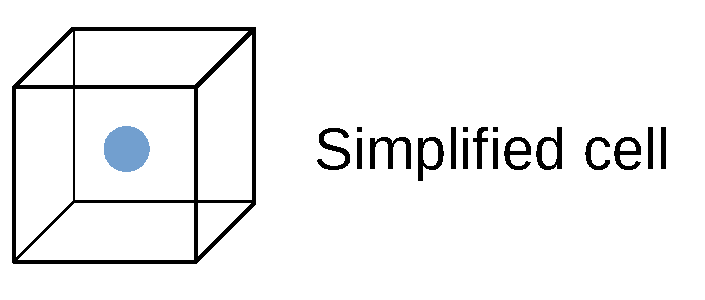
\includegraphics[height=1.5cm]{figs/Simplified_cell.pdf}
            %\end{figure}
    \normalsize
             \vspace{-3em} 
    	    \begin{figure}
               \centering
               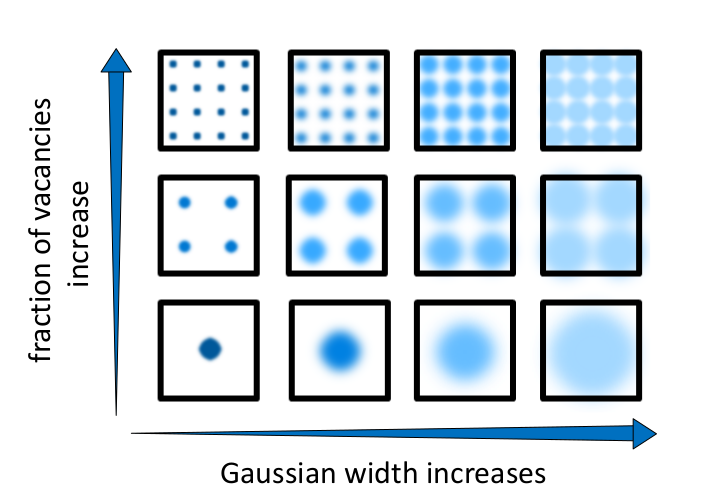
\includegraphics[height=4.5cm]{VaryWidthandVacancies}
               %\caption{Number density profiles $n(\vec r)$, all with 
               %the same number density, n.}
            \end{figure} 
             %\vspace{-0.5em} 
                \footnotesize
    $~~~~~~~~~~~~~~~~~$Number density profiles $n(\vec r)$ 
  
    $~~~~~~~~~~~~~~~~$for a given number density, n 
    
    $~~~~~~~~~~~~~~~~~~~~~~~~~$and temperature
	\end{columns}
\end{frame}


\section*{WCA Phase diagram}
\subsection{WCA Temperature-Density Phase Diagram}
\begin{frame}{Temperature-Density Phase Diagram}
\begin{columns}
    \column{.5\textwidth}
	    \vspace{-3em}
        \begin{block}{}
            \begin{itemize}
              \item Data shown for temperatures from $K_BT=~$0.5 to 3.0
              \item Freezing indicated by 
            
               presence of coexistence
            
               region where an abrupt
               
               change in density occurs
              
              \item Close match with 
              
              Monte-Carlo simulations!
            \end{itemize}
            \end{block}
       \column{.65\textwidth}
    \begin{figure}
        \centering
        \includegraphics[width=.9\columnwidth]{figs/Phase_Diagram_of_T_vs_n}\\
    \end{figure}        
    \vspace{-1em}
    \footnotesize $~~~~~~~~$White lines are Monte-Carlo data from  
    
     $~~~~$Christopher May's OSU undergraduate thesis
     \normalsize
     \end{columns}
\end{frame}

\end{document}






